\section{Adaptive Counting Rule Duplication}\label{sec:dup}
\subsection{Counting Rule Duplication Problem}\label{sec:dup-prob}
Recall the 80/20 rule indicating only a small portion of flows are elephant flows, duplicating all the counting rules will waste lots of flow entries.
A straightforward method is to adaptively duplicate the counting rules for those flows that cannot be counted in their original switches.
However, considering there could be multiple flows requiring extra counting rules simultaneously, the arbitrary duplication may produce the hot spot where the switch runs out of its flow table entries and/or counting memory.
That is, we must carefully decide where to duplicate the rule for each flow, namely counting rule duplication problem (CRDP).

We formalize CRDP as follows.
Assume there are $N$ switches in total, and $M$ flows requiring extra counting rules.
If we duplicate a counting rule for flow $M_i$ to switch $N_j$, it will consume $a_{ij}$ counting memory along with $b_{ij}$ flow table entries.
If $M_i$ cannot be assigned to $N_j$, \ie, $N_j$ is not in the routing path of $M_i$, $a_{ij}$ and $b_{ij}$ will be infinite.
Note that $b_{ij}$ does not always equal to 1, because the counting rule may have to be further divided to fit into the original flow table.
In sum, CRDP can be formalized by the following model:
\begin{eqnarray}
\text{minimize}  & \displaystyle\sum\limits^{M}_{i=1} a_{ij}x_{ij}\sum\limits^{M}_{i=1} b_{ij}x_{ij} & j=1,...,N\\
\text{subject to}& \displaystyle\sum\limits^{M}_{i=1} a_{ij}x_{ij}\leq A_j,  & j=1,...,N \\
                 & \displaystyle\sum\limits^{M}_{i=1} b_{ij}x_{ij}\leq B_j,  & j=1,...,N \\
                 & \displaystyle\sum\limits^{N}_{j=1}x_{ij}=1,  & i=1,...,M
\end{eqnarray}

Eq. (1) is to minimize the cost of counting memory and flow entries.\footnote{The weights of the two parts are unknown, so we multiply (not add) them.}
Eq. (2) and Eq. (3) constrain the counting memory and number of flow entries.
Eq. (4) defines a 0-1 variable to represent that each rule can only be duplicated to one switch.
Actually, $a_{ij}$ is a constant value for all assignment ($M_i$ to $N_j$), since DIAL allocates same-size counters for each flow.
As a result, we could rewrite the objective to minimize the second factor, \ie, the number of flow entries.
In this way, CRDP captures the well-known Multi-Resource Generalized Assignment Problem (MRGAP), which has been proved to be NP-hard~\cite{doi:10.1287/mnsc.37.6.695}.

We note that $M$ could be relatively small in practice due to the limited number of elephant flows.
However, the first-time ``duplication'', \ie, the initial counting rule placement, involves all flows in the network, incurring a large overhead of computing optimal solution.
As a result, we still need to seek near-optimal solution for CRDP.

\subsection{Heuristics of Near-Optimal Duplication}\label{sec:dup-alg}
Due to the NP-hardness of CRDP, we propose some simple heuristics to approximately approach the optimal duplication solution under the acceptable time consumption.
Specifically, we consider the following requirements of duplication placement:
(1) the consumption of the two resources (counting memory and \#flow entries) should not go beyond their capacities, and
(2) the consumption of the two resources should be balanced for all switches.

The heuristics is to greedily find the lightest-loaded switch to duplicate the counting rule for each flow that exceeds its original counter, namely Lightest-Loaded-First duplication (LLF).
We note that, for a certain flow, the number of candidate switches for duplication is actually the number of hops of this flow.
That is, flows with longer path have more options to place the duplicated rules.
As a result, for a bunch of flows to be duplicated, LLF will first decide the duplication place for the flows with shorter path.

Algorithm~\ref{alg:place} depicts the whole process of finding a near-optimal duplication solution.
To be specific, \texttt{multi\_place} works out the priority of all the duplicating flows by their routing paths' length, and \texttt{place} finds the lightest-loaded switch from the candidates for each duplicating flows sequentially.

For example in Fig.~\ref{fig:exam-dial-place}, each switch counts four flows in the beginning.
Suppose that the routing paths of $f_1$ and $f_2$ are $S_1 \rightarrow S_2$ and $S_1 \rightarrow S_2\rightarrow S_3$, respectively.
If afterwards both $f_1$ and $f_2$ in $S_1$ need to duplicate their counting rules, \texttt{multi\_place} will first arrange to \texttt{place}($f_1$) that has a shorter routing path.
For $f_1$, only $S_2$ is available, so it duplicates the rule to and creates a 1-bit counter in $S_2$.
Next, \texttt{place}($f_2$) is called, and here $S_3$ is lighter loaded than $S_2$, so the duplicated rule will be placed in $S_3$.

\begin{figure}
    \centering
    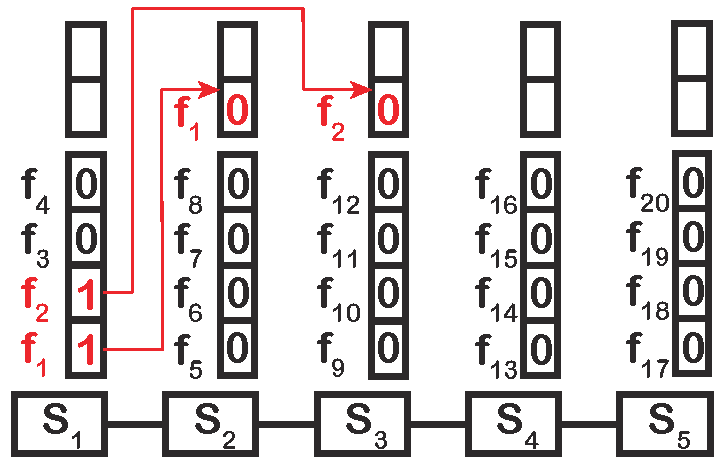
\includegraphics[width=0.6\linewidth]{pic/exam-dial-place.pdf}
    \caption{Example of the duplication for DIAL.}
    \label{fig:exam-dial-place}
\end{figure}

\begin{algorithm}[t]\small
\caption{Lightest-loaded-first duplication}
\label{alg:place}
\KwIn{\KwOut{the set of flows to be duplicated: $fs$}}
\BlankLine
\texttt{multi\_place}($fs$)
\Begin{
     sort $fs$ in ascending order of the number of available switches along the routing path of each flow\;
    \ForEach{$f\in fs$}{\texttt{place}($f$)\;}
}
\BlankLine
\texttt{place}($f$)
\Begin{
    $ss \leftarrow$ \{$s$ $|$ $s$ is along the routing path of $f$ and there is no rule of counting $f$ in $s$\}\;
    sort $ss$ in ascending order of the load of each switch\;
    $lis \leftarrow$ the lightest-loaded switch of $ss$\;
    install the rule of counting $f$ in $lis$\;
    create the counter of $f$ in $lis$\;
}
\end{algorithm}

\textbf{Pre-duplication.}
Ideally, the duplication happens only when the original counter exceeds.
However, this process has to wait for the controller to issue the new counting rule, which will incur large latency through each duplication.
We employ a pre-duplication process into DIAL to mitigate the latency problem.
Specifically, after initially placing the counting rules, we directly duplicate them by re-running \texttt{multi\_place} of LLF in Algorithm~\ref{alg:place}.
That is, all the counting rules are at least duplicated once.
When a flow exceeds its first counter, a third one will be allocated immediately.
As a result, the controller has plenty of time to issue the new counting rule, as long as the second counter is not full.
In this way, elephant flows are properly counted without employing extra latency.

Fig.~\ref{fig:exam-dial-predup} depicts a possible result after the pre-duplication, in which the assumptions are the same as those in Fig.~\ref{fig:exam-dial-dmn8}.
After duplicating all the counting rules once, each switch counts eight flows now.
It can be seen that $f_1$ has two counters in $S_1$ and $S_2$ at the start, and the one in $S_1$ is counting the first byte of $f_1$.
When $f_1$ exceeds its counter in $S_1$, \texttt{overflow\_report} in Algorithm~\ref{alg:handle} will \texttt{place}($f_1$) in another switch, $S_3$. Meanwhile, the elephant flow $f_1$ can be properly and continuously counted in $S_2$.

\begin{figure}
    \centering
    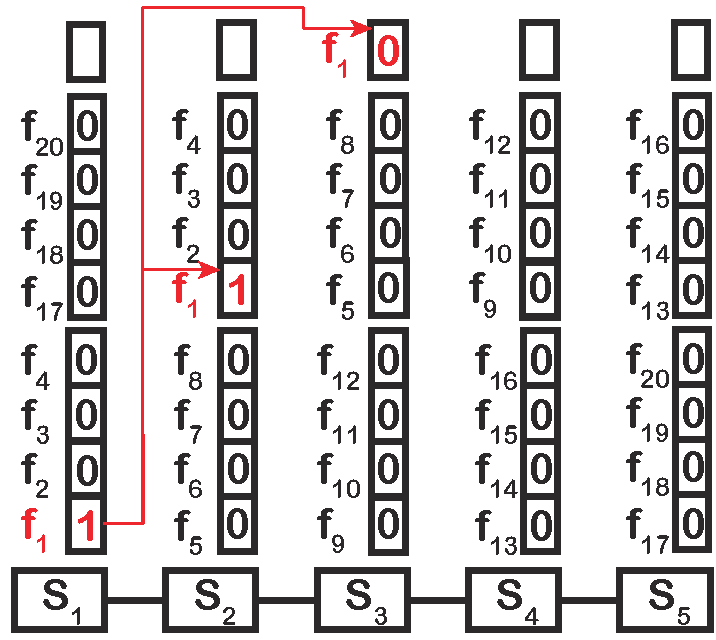
\includegraphics[width=0.6\linewidth]{pic/exam-dial-predup.pdf}
    \caption{Example of the pre-duplication for DIAL.}
    \label{fig:exam-dial-predup}
    \vspace{-0.1in}

\end{figure}
